
\newpage
\chapter{Formules}

\section{Tableau Trigonométrique}
\begin{tabular}{|l|c|c|c|c|c|c|}
  \hline
  Degree & $0^{\circ}$ & $30^{\circ}$ & $45^{\circ}$  & $60^{\circ}$ & $90^{\circ}$ \\
  Radians & 0 & $\frac{\pi}{6}$ & $\frac{\pi}{4}$ & $\frac{\pi}{3}$ &  $\frac{\pi}{2}$ \\
  \hline
  sin & 0 & $\frac{1}{2}$ & $\frac{\sqrt{2}} {2}$ & $\frac{\sqrt{3}} {2}$ & 1 \\
  cos & 1 & $\frac{\sqrt{3}} {2}$ & $\frac{1}{2}$ & $\frac{\sqrt{2}} {2}$ & 0 \\
  tan & 0 & $\frac{\sqrt{3}} {3}$ & 1 & $\sqrt{3}$ & $\nexists$ \\
  cotan & $\nexists$ & $\sqrt{3}$ & 1 & $\frac{\sqrt{3}} {3}$ & 0 \\
  \hline
\end{tabular}

\vspace{4mm} %5mm vertical space
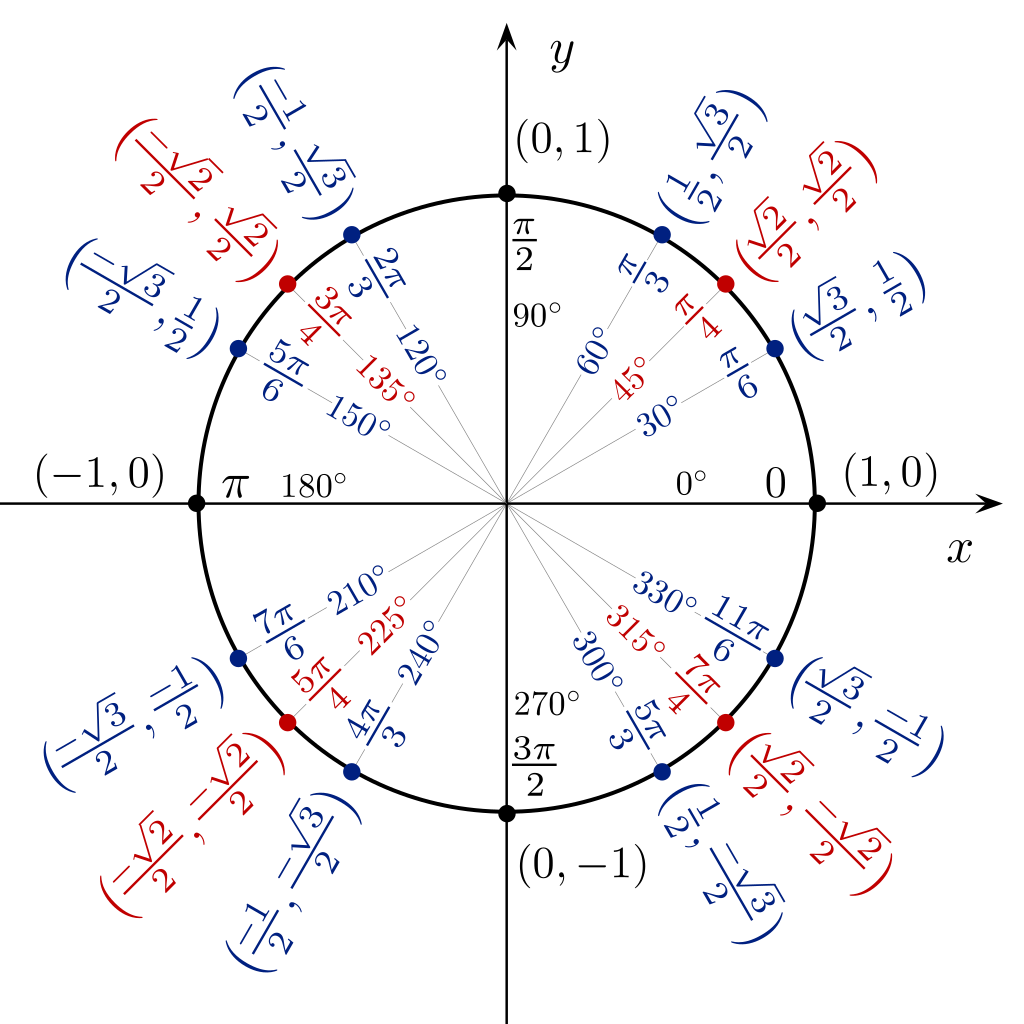
\includegraphics[scale=0.3]{circle_angles}


\newpage
\vspace{4mm} %5mm vertical space
\section{NB Complex : Cartésienne vers Polaire}
$\rho = \sqrt{x²+y²}$ \\
$\theta = arctg(\frac{Y}{X})$ \\
$\frac{Y}{X} = tg(\theta)$ \\

\vspace{4mm} %5mm vertical space
\section{NB Complex : Polaire vers Cartésienne}
$X= \rho * cos(\theta)$ \\
$Y= \rho * sin(\theta)$ \\
$Z= x+yi $ \\
Notes : $cis = cos(\theta) * sin(\theta) *i$ \\

\vspace{4mm} %5mm vertical space
\section{Addition de nombre complex}

$tg = \frac{sin}{cos}$ \\
$\theta = arctg(\frac{Y}{X})$ \\

$ Exemple : 4*cis(45^{\circ}) + 5*cis(\frac{\pi}{3})$\\

$\rho = \sqrt{\rho_1^{2}+\rho_2^{2} + 2 * \rho_1 * \rho_2 * cos(\theta_1-\theta_2))}$ \\

$\theta = arctg(\frac{Y}{X})$\\

$\theta = arctg(\frac{\rho_1 * sin(\theta_1) + \rho_2 * sin(\theta_2)} {\rho_1 * cos(\theta_1) + \rho_2 * cos(\theta_2)})$ \\

\vspace{4mm} %5mm vertical space
\section{Soustraction de nombre complex}

$\theta = arctg(\frac{Y}{X} => tg = \frac{sin}{cos} )$ \\

$ Exemple : 4*cis(45^{\circ}) + 5*cis(\frac{\pi}{3})$\\

$\rho = \sqrt{\rho_1^{2}+\rho_2^{2} + 2 * \rho_1 * \rho_2 * cos(\theta_1-\theta_2))}$ \\

$\theta = arctg(\frac{Y}{X})$\\

$\theta = arctg(\frac{\rho_1 * sin(\theta_1) + \rho_2 * sin(\theta_2)} {\rho_1 * cos(\theta_1) + \rho_2 * cos(\theta_2)})$ \\

\vspace{4mm} %5mm vertical space
\section{Multilication de nombre complex}

$\theta = arctg(\frac{Y}{X} => tg = \frac{sin}{cos} )$ \\

$ Exemple : 4*cis(45^{\circ}) + 5*cis(\frac{\pi}{3})$\\

$\rho = \sqrt{\rho_1^{2}+\rho_2^{2} + 2 * \rho_1 * \rho_2 * cos(\theta_1-\theta_2))}$ \\

$\theta = arctg(\frac{Y}{X})$\\

$\theta = arctg(\frac{\rho_1 * sin(\theta_1) + \rho_2 * sin(\theta_2)} {\rho_1 * cos(\theta_1) + \rho_2 * cos(\theta_2)})$ \\


\vspace{4mm} %5mm vertical space
\section{Division de nombre complex}

$\theta = arctg(\frac{Y}{X} => tg = \frac{sin}{cos} )$ \\

$ Exemple : 4*cis(45^{2}) + 5*cis(\frac{\pi}{3})$\\

$\rho = \sqrt{\rho_1^{2}+\rho_2^{2} + 2 * \rho_1 * \rho_2 * cos(\theta_1-\theta_2))}$ \\

$\theta = arctg(\frac{Y}{X})$\\

$\theta = arctg(\frac{\rho_1 * sin(\theta_1) + \rho_2 * sin(\theta_2)} {\rho_1 * cos(\theta_1) + \rho_2 * cos(\theta_2)})$ \\

\section{Logique propositionnelle}

\vspace{5mm} %5mm vertical space
De Morgans: \\
a v b= ¬a * ¬b\\
a*b= ¬a + ¬b\\
(p∧q) = ¬p v ¬q  \\
(pvq) = ¬ (¬p ∧ ¬q)  \\
¬(p∧q) = (p v q)  \\
(A ∧¬ B) V (¬ A V (C ∧ A)) =  ¬(A ∧¬ B) ∧ ¬(¬ A V (C ∧ A))\\

\vspace{5mm} %5mm vertical space
Forme conjonctive: \\
(A ET B) OU C \\
(A ∧ B) V C\\

\vspace{5mm} %5mm vertical space
Forme disjonctive : \\
(A OU B) ET C \\
(A V B) ∧ C\\

\vspace{5mm} %5mm vertical space
Transformation: \\
A$=>$B = ¬A v (A∧B) \\
A$<=>$B: = (A$=>$B)∧(B$=>$A)  \\
(A$=>$B)∧(B$=>$A) = (¬A v (A∧B)) ∧ (¬B v (B∧A))
